\section{Cosmic muon telescope and Micromegas octuplet}
\label{sec:exp}

The Micromegas and scintillator detectors of the Harvard cosmic ray test stand are described in detail in previous notes presenting 
the performance of the full MMFE8 readout~\cite{noisy,noiseless}. Eight layers of Micromegas detectors are stacked vertically for the
 purpose of providing eight measurements of the position of a cosmic muon as it travels through the experiment.
 The readout strips of each layer have a 0.4 mm pitch, and are arranged according to the NSW design: $XXUV-UVXX$, in which strips in the $X$ planes run
 perpendicular to the readout edge of the chamber, and strips in the $U$ ($V$) planes are tilted at
 an angle of $1.5^\circ$ ($-1.5^\circ$) to provide a measurement of the non-precision $y$ coordinate. Each Micromegas detector covers an active area of
 200 x 204.6 mm$^2$.
The type and $z$~position of the different readout
 planes are summarized in Table~\ref{tab:tab_1}.
%%%%%%%%%%%%%%%%%%%%%%%%%%% 
\begin{table}
 \begin{center}
% \begin{ruledtabular}
 \begin{tabular}{lccc}
 \hline \hline
  Readout plane  &  Type & $z_{\rm board} (mm)$ &  $z_{\rm bary} (mm)$      \\
  0      & $X$   &  0.0 &  -2.7     \\ 
  1      & $X$  & 11.2 &   13.9  \\
  2      & $U$   &32.4 &   29.7 \\
  3      & $V$   & 43.6 &    46.3   \\
  4      & $U$   & 113.6 &    110.9    \\
  5      & $V$   & 124.8 &   127.5  \\
  6      & $X$   & 146.0 &    143.3   \\
  7      & $X$   & 157.2 &    160.0   \\
 \hline \hline
 \end{tabular}
% \end{ruledtabular}
 \caption{ Characteristics of the 8 Micromegas planes assembled into 2 quadruplets (see text).
 Planes $x$ have electrodes parallel to the scintillator $x$ coordinates. Electrodes of planes $u$ and $v$ are 
tilted with respect to the $x$ electrodes by $\pm 1.5 \deg$, respectively. The  positions
along the $z$ axis of each electrode plane are called  $z_{\rm board}$. 
The $z$ position at half drift gap, where the barycenter is reconstructed, is called $z_{\rm bary}$. 
 }
\label{tab:tab_1}
 \end{center}
\end{table}
Three layers of scintillators counters -  placed above, on top, and below the octuplet -  provide a trigger
for the full MMFE8 readout. A scintillator trigger requires the coincidence of signals in all three layers. 
 Concrete blocks, 5 feet thick, are placed between the octuplet and the bottom scintillator to harden the muon sprectrum.

\subsection{Readout electronics}
\label{sec:exp-elx}
The Micromegas readout electronics consists of three cards. The MMFE8 card is a demonstrator that houses 8 VMM2 ASICs per card.
 These ICs provide digitized  arrival-time and charge information for the signal of each  Micromegas readout strip.  
 A description of the MMFE8 boards can be found in Refs.~\cite{noisy,mmfe8}. A study of its performance is in
 Refs.~\cite{noisy,noiseless}. The MMFE8 demonstrator uses a FPGA for configuring
 and reading out the VMMs digitized information  over ethernet.
 We use 8 MMFE8s to read the 512 channels of  the 8 layers of Micromegas in the octuplet.

 The ADDC card~\cite{nswtdr} receives data from 4 MMFE8s over miniSAS connections and packages this data
 into a single output for the MMTP board. For this purpose, the ADDC V1 uses a FPGA communicating with a GBTx chip.
 As mentioned earlier, we need two such boards.

The Micromegas Trigger Process (MMTP) is the last card of the Micromegas trigger path. It receives data from ADDCs over SFP+  optical connections and
 searches the data for the presence of hits consistent with a track segment using firmware running on a  VC707 FPGA evaluation board.
  Pictures of the ADDC V1 and the demonstrator MMTP are shown in Figure~\ref{fig:cards}.

\begin{figure}[!htpb]
  \begin{center}
    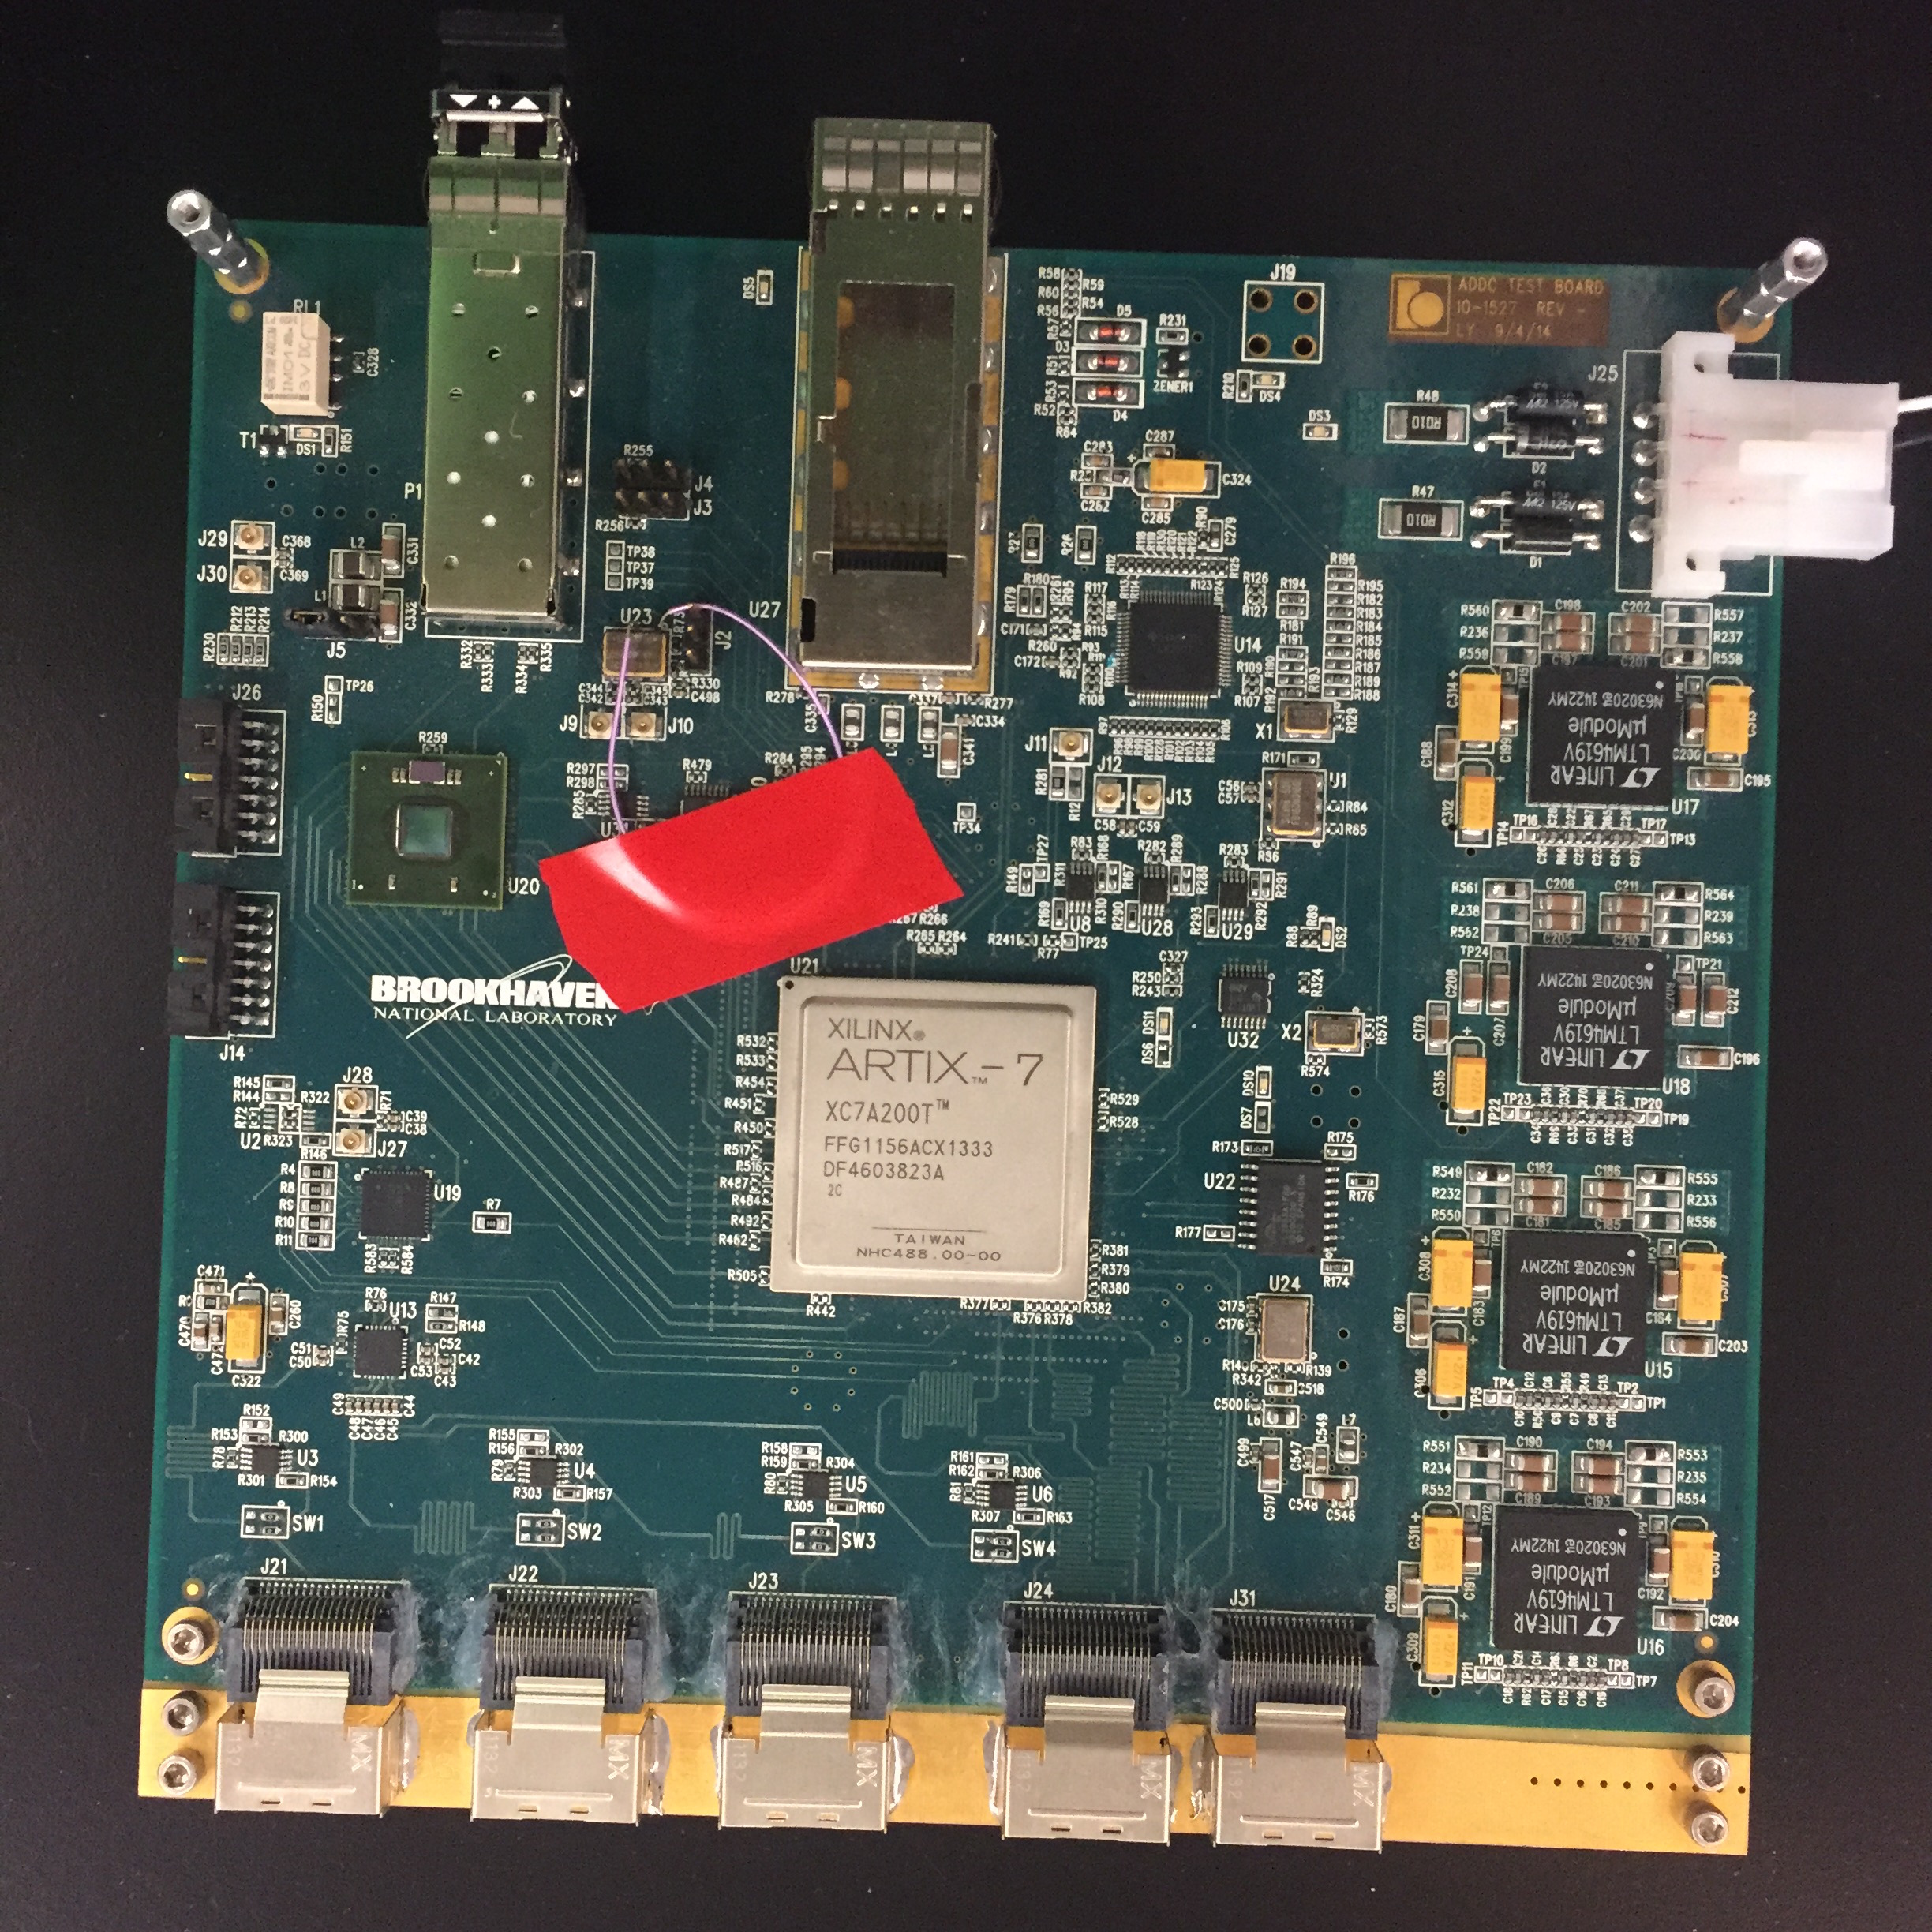
\includegraphics[width=0.48\textwidth]{figures/photos/IMG_0840.JPG}
    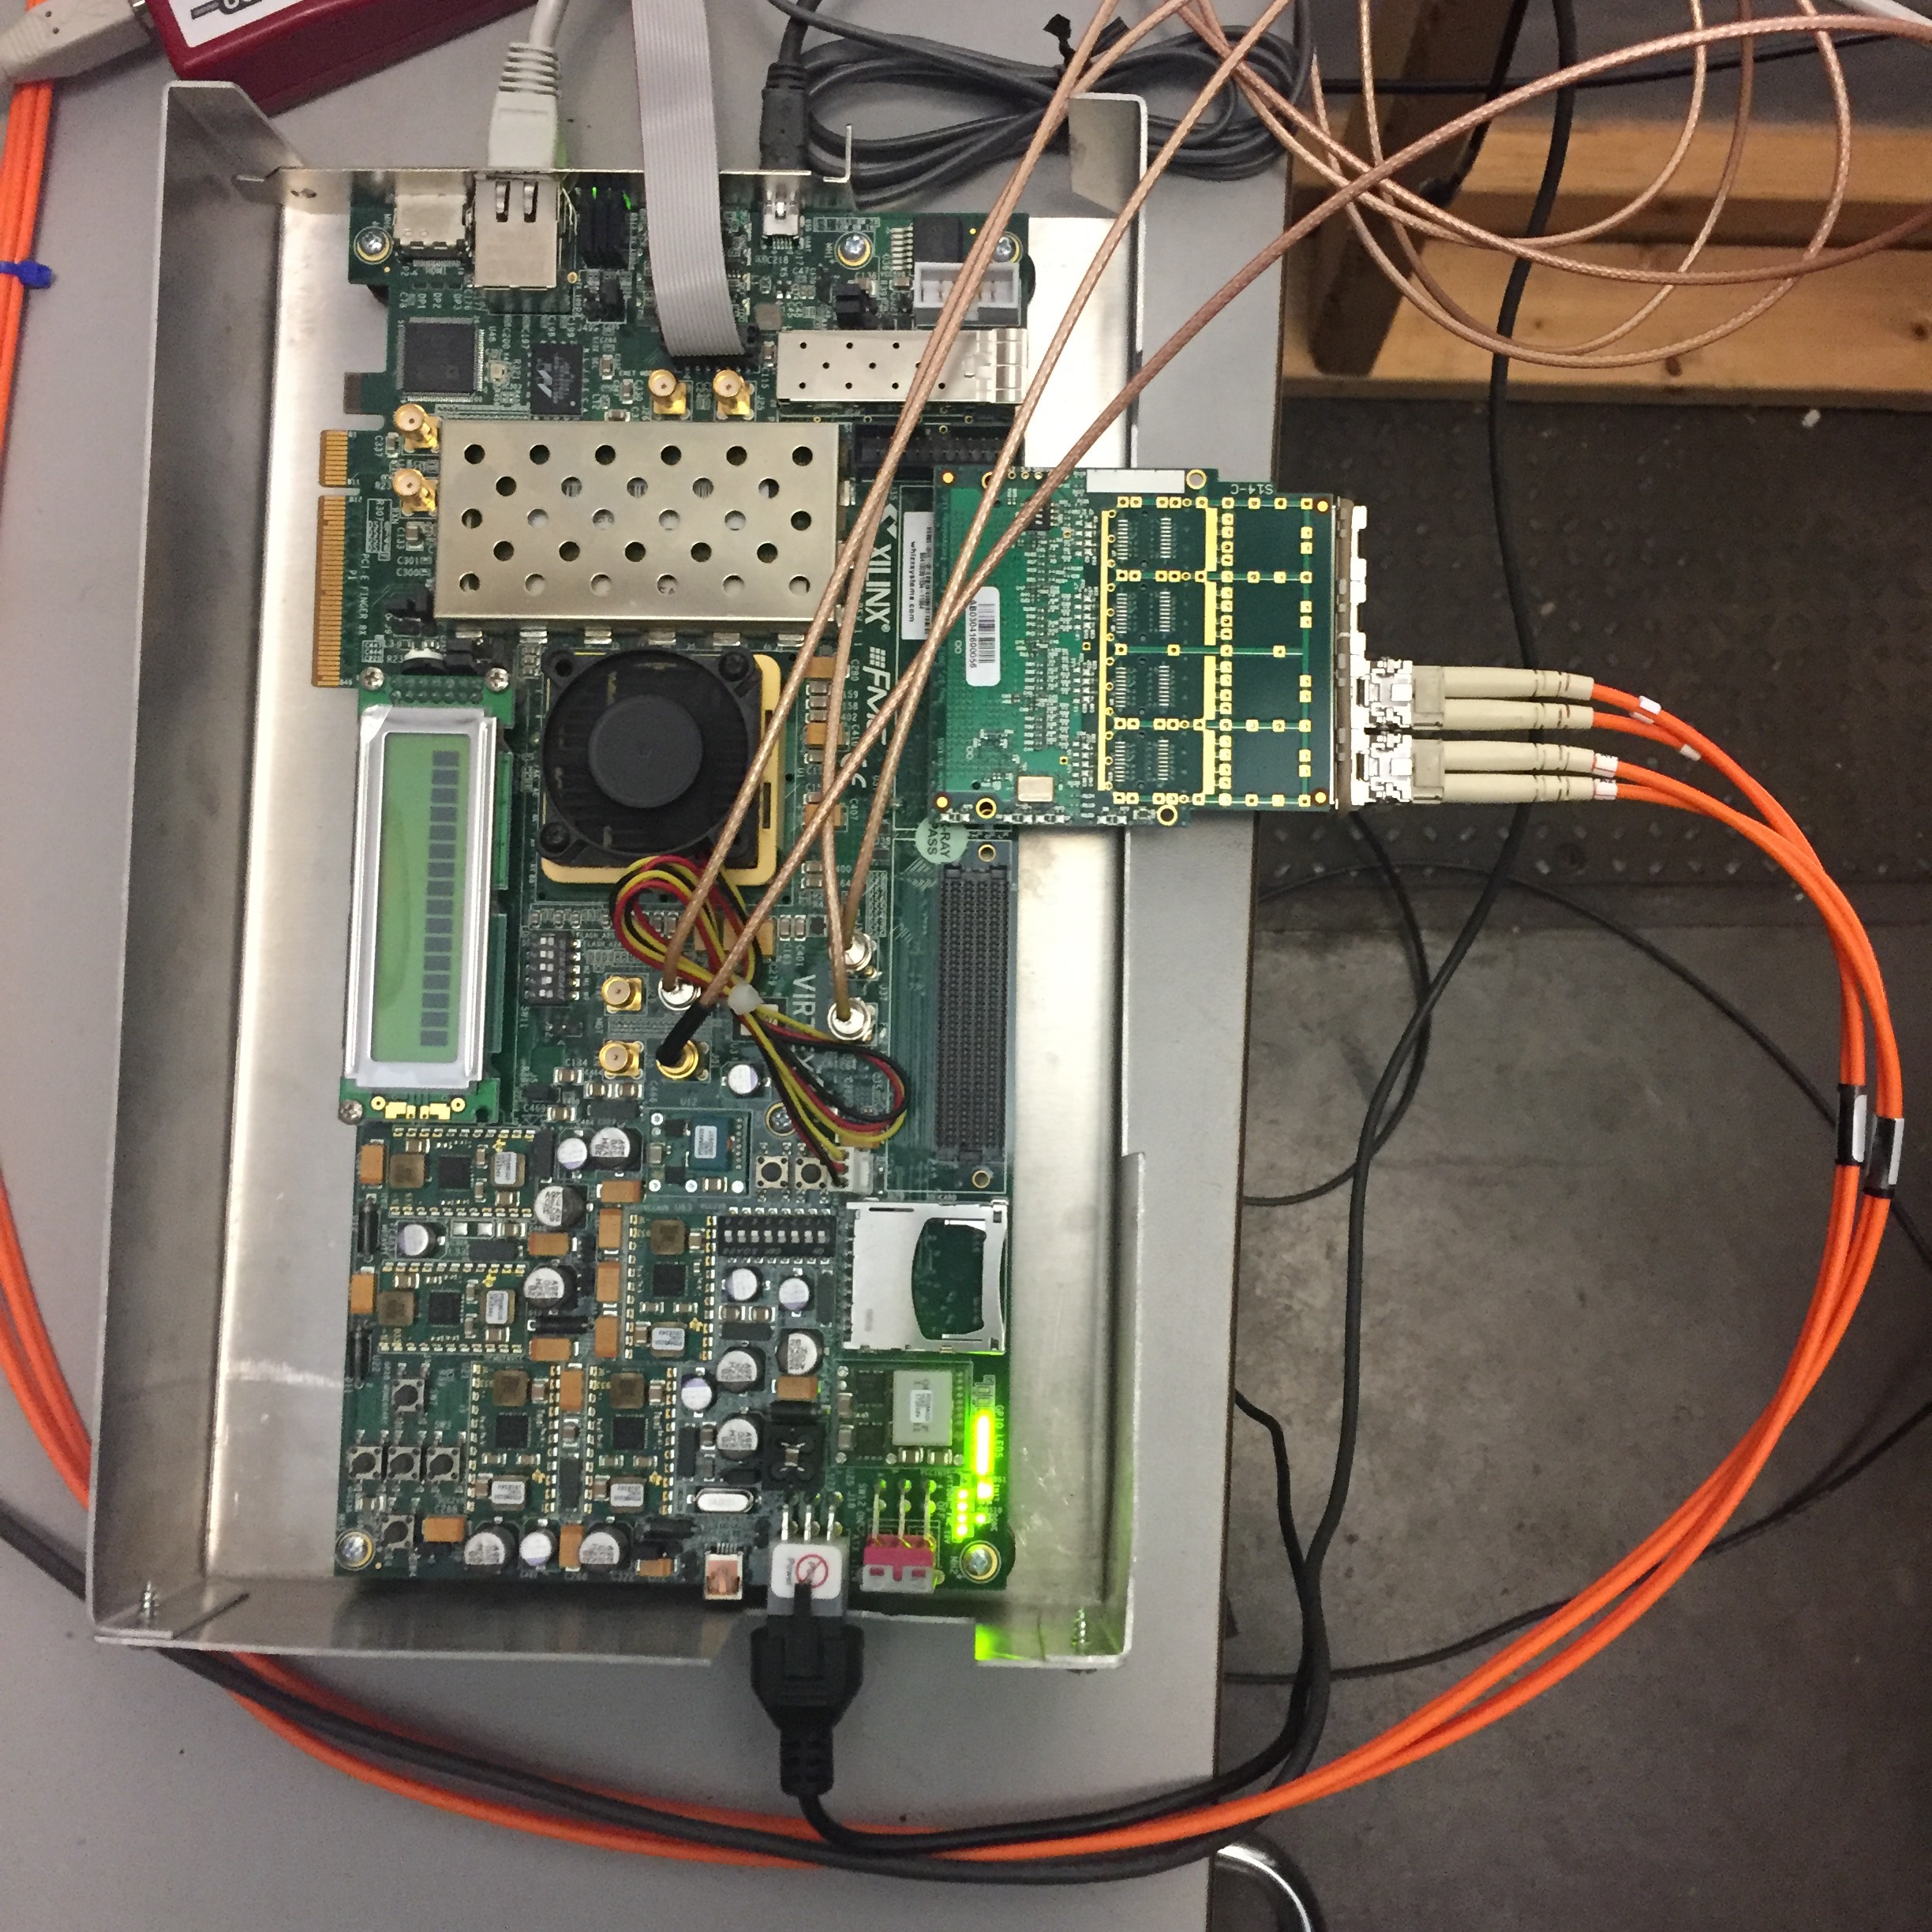
\includegraphics[width=0.48\textwidth]{figures/photos/IMG_0836.JPG}
  \end{center}
  \vspace{-10pt}
  \caption{Pictures of the ADDC V1  (left) and the MMTP board (right).}
  \label{fig:cards}
\end{figure}

An additional board, referred to as  clock/trigger card, has been designed  by J.~MacArthur.
 This board generates and distributes a 40 MHz clock to all MMFE8 and MMTP boards.
 Time is measured in units of BC, where BC is a tick of this clock.
 The content of counters incremented using this common external clock, referred to as BCID and
 located in all boards, is attached to the event information.
The clock/trigger cards also receive and distribute scintillator-trigger signals   
as discussed in Section~\ref{sec:exp-mmfe}. 
A  flow diagram of the hardware is shown in Figure~\ref{fig:cartoon_elx}.

\begin{figure}[!htpb]
  \begin{center}
    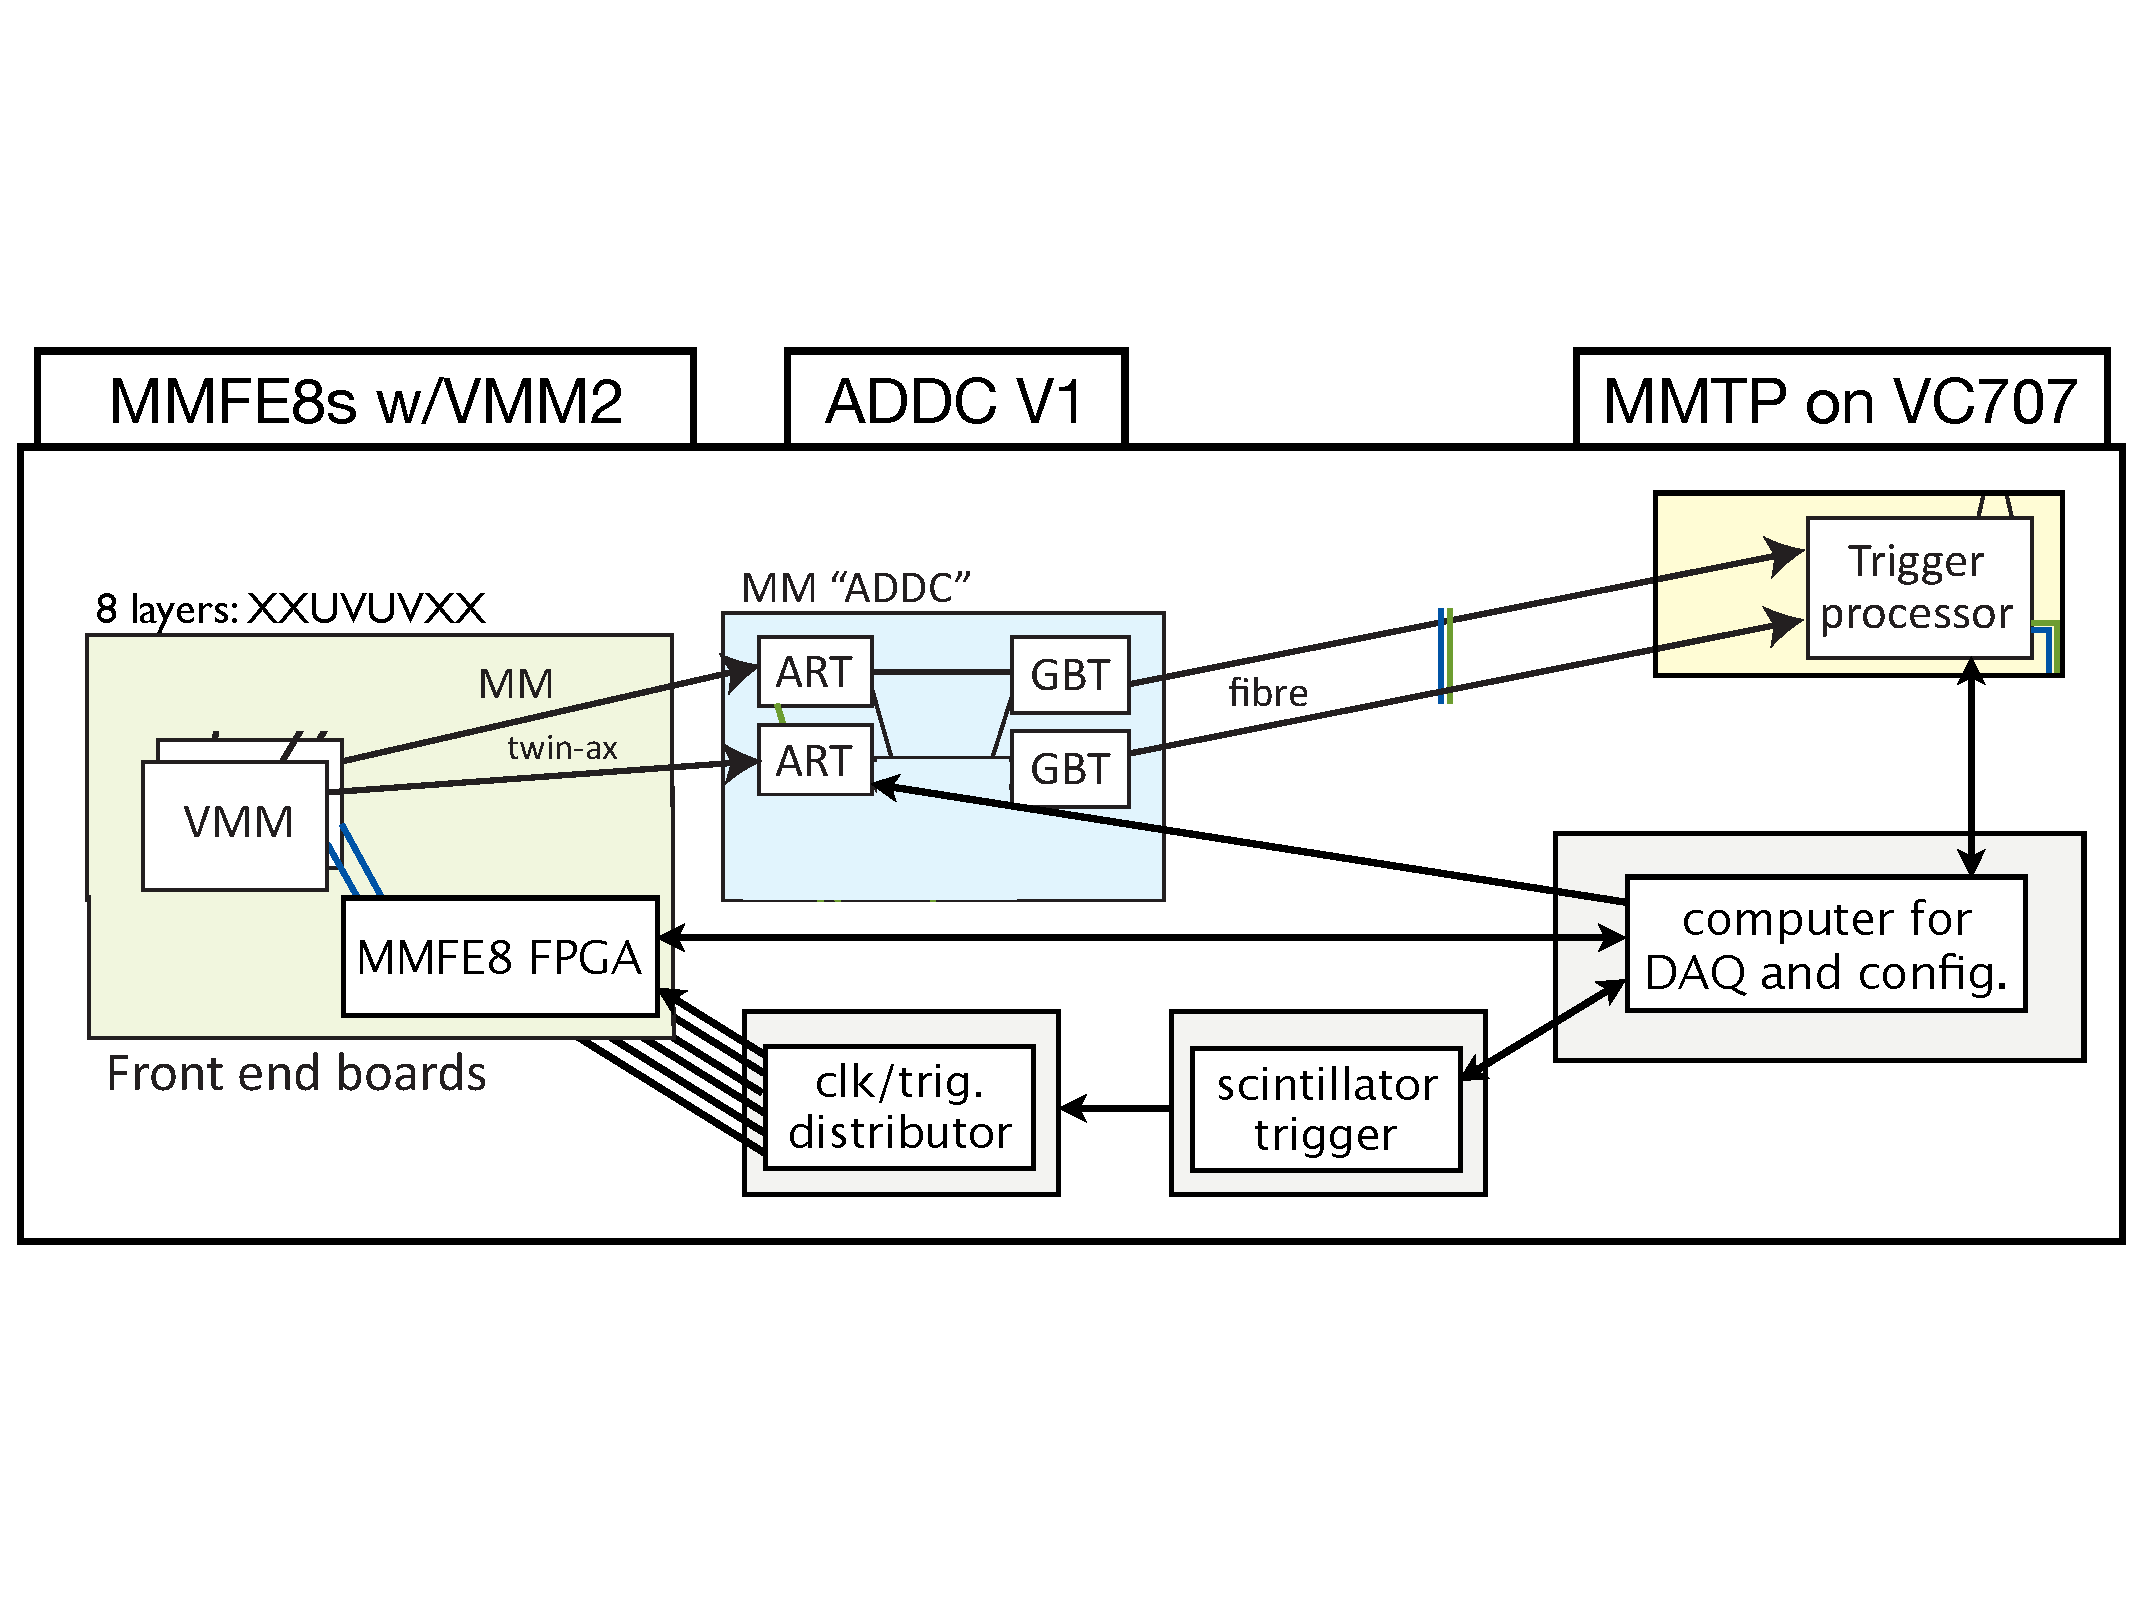
\includegraphics[width=1.0\textwidth]{figures/cartoons/electronics_path.pdf}
  \end{center}
  \vspace{-20pt}
  \caption{Schematic of the data flow in the readout electronics used at the Harvard cosmic ray test stand. 
    Inspiration for the cartoon was provided by L. Levinson.}
  \label{fig:cartoon_elx}
\end{figure}

\subsection{Trigger data path}
\label{sec:exp-art}

The MMTP data path starts with the ART signal provided by each VMM.
The VMM has two operating modes for the ART signal: the ART flag can be issued when the integrated charge of a signal is above threshold ($\simeq$ 3 fC) or reaches its peak value 
 ($\simeq$ chosen peaktime, usually 200 ns). We choose the first mode to reduce the latency of the Micromegas trigger which is already
 quite close to the allocated 1 $\mu$s~\cite{nswtdr}.

The ART flag is followed by the serialized address of the channel (6-bits) released at rising and falling edges of the
 MMFE8 160 MHz ART clock,  derived by boosting up  the external BC clock.
At the flag falling edge,
the ADDC uses the MMFE8 ART clock to deserialize the ART address. This clock, scaled down to 40 MHz, also increments a counter, the value of which
at the flag  is attached to the channel address together with  MMFE8 board and VMM numbers (ART string). 
 At each  BC, the ADDC uses  GBTx frames to collapse the ART informations of 32 VMMs into 112-bits packets which
are sent through a SFP+ optical link to the MMTP board. Each frame has only space for 8 ART strings. If more strings are present,
 the ADDC keeps the eight with highest priority, where the priority is assigned according to the VMM position. While this is not a problem in our case,
this step will need re-evaluation in the LHC high-L situation.

 The  e-link between each MMFE8 and the ADDC is provided by miniSAS 36-line cables in which each VMM ART output uses a preassigned pair of cables.
 Unfortunately, the ART clock uses pairs of  unshielded sideband lines which generate quite a bit of
 EMI captured by the octuplet Al frame and in turn injected into the Micromegas readout electrodes.
 It took us a few months to discover it and one day to fix it.

  



  The ADDC V1 were built by BNL and the firmware to receive the data, align  and format them was imported by Lin Yao from the ART ASIC
architecture\cite{addc}.
 Two mistakes were found and fixed in the firmware: a) an error in deserializing ART data with the 160 MHz clock which produced
 incorrect ART addresses; and b) the ART flag, variable in length, was not always detected resulting into a loss of events.
 Other than that, the ADDC firmware was found to be flawless.
 The MMTP process uses the ADDC information to find and characterize trigger candidates.   

 
As in the NSW design, the 2 ADDCs are placed near the octuplet and the VC707 board receiving
 their data is placed in a 10 m away shack -elevated to control room status- 
 which also houses the DAQ computer and scintillator trigger/readout electronics. 

\subsection{MMFE8 and scintillator data path}
\label{sec:exp-mmfe}
The ART data is distinct from the full readout of the MMFE8, as the latter includes detailed information about the charge and arrival
time of all signals captured during one event. This event information is used to evaluate the MMTP efficiency, and
time and spatial resolution independently of the octuplet efficiency.
The MMFE8 and scintillator data paths are described in detail in Refs.~\cite{noisy,noiseless}. Upon a scintillator trigger, the DAQ computer pulls out 
 the MMFE8 information recorded  in 100 $\mu$s before the trigger using an ethernet connection. 
 The arrival time of the scintillator signals are also recorded
 and sent over ethernet to the DAQ computer. Micromegas and scintillator data, as well MMTP data, are recorded event by event with the DAQ-computer time stamp.
 This allows us to recombine the information of a single event split into different files. 

 The scintillator trigger, which has a 1.2 ns resolution, is also sent to the MMTP where it is stamped with content of a counter incremented by  the  640 MHz 
clock derived from  the external BC clock.




